\section{Outlook and guidance for future separators}

\subsection{Recoil separators planned and under construction}

At the time of writing, there are a handful of recoil separators being constructed or in the conceptual or design phase at laboratories worldwide. It is not the intention of the authors to summarize all of these proposals, as some of these may evolve in design, switch scientific focus, or indeed not be funded. However there are a couple of developments worth mentioning here, specifically projects that are aimed at astrophysics and are under detailed design or construction now. 

St. George (Strong Gradient Electromagnetic Online Recoil separator for capture Gamma Ray Experiments) \cite{cou08} is a recoil separator under construction at the Institute for Structure and Nuclear Astrophysics at the University of Notre Dame. The design is optimized for the study of astrophysical low energy ($\alpha,\gamma$) reactions for up to A=40 beam mass. The beams will be provided by the new 5MV accelerator at the laboratory. The separator has design acceptance values of $\pm$40 mrad in angle and $\pm$7.5\% in energy. It is built in a configuration providing selection of a single charge state via magnetic analysis, before mass separation is performed in a Wien filter (see figure \ref{fig:stgeorge}), with a final resolving power of $m/\Delta m=100$. It is designed to have high a beam suppression factor of $\ge10^{15}$. In particular the Wien filter element of this separator is specially optimized to improve the filtering efficiency, achieved by minimizing the magnetic dipole component fringe fields and by incorporating specially-shaped electrodes so that the electric fringe fields closely follow the magnetic ones. 

The Separator for Capture Reactions (SECAR) is a recoil separator design destined to be a flagship experiment at the Facility for Rare Isotope Beams (FRIB)  at the National Superconducting Cyclotron Laboratory (NSCL) at Michigan State University. The present design is based on the St. George separator, but using an additional Wien filter \cite{ber10}. The separator will operate using reaccelerated radioactive ion beams produced by fragmentation at FRIB and prepared using a gas stopper system. The scientific purpose of this experiment is to continue the study of proton- and alpha- induced radiative capture reactions for explosive nucleosynthesis and represents an important part of the US nuclear physics community's long range plan. The JENSA jet gas target mentioned in section \ref{gas} \cite{chi13} is planned for use with the SECAR separator. 

\begin{figure}
\resizebox{0.9\columnwidth}{!}{
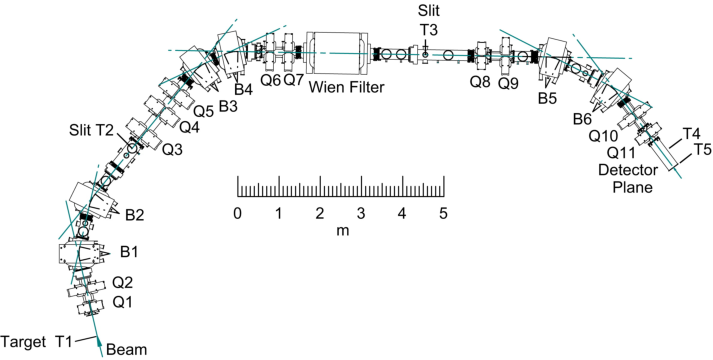
\includegraphics{stgeorge}
}
%\vspace{5cm}       % Give the correct figure height in cm
\caption{Schematic view of the St. George separator. Taken from \cite{cou08}.}
\label{fig:stgeorge}
\end{figure}



\subsection{Suggested avenues of technical development} 

\subsubsection{Acceptance}

\subsubsection{Rigidity}

\subsubsection{Operation}

\subsubsection{Detection}